% (M5-M24) Leader: NCSR "D"
% CeADAR, UPC, ATOS, EVIDEN, FDI, INRIA, ARCADA, use case partners

\subsection{Introduction}

In this research, we aim to develop a task-agnostic framework for time-series data quality estimation. Towards this goal, we propose methods for anomaly and noise detection, which allow us to identify biased, noisy, inconsistent, or otherwise low-quality data, as well as data that may have been maliciously manipulated to contaminate the model during training.

As a case study to validate our methods, we use the Bitbrain dataset, which consists of EEG signals collected from a headband across 128 recordings. This headband includes two EEG channels synchronized with medical-grade EEG devices. The signals are annotated by three experts, with each 30-second segment classified into one of five sleep stages: Wake, N1, N2, N3, and REM. These stages correspond to specific brain activity patterns, such as slow eye movements, sleep spindles, and other characteristic waveforms.

To further validate the robustness of our proposed methods, we explore data augmentation techniques, including adversarial machine learning methods that introduce controlled noise contamination into the dataset.

\subsection{Problem Statement}

The quality of time-series data plays a crucial role in the performance of machine learning models, yet existing methods often fail to effectively identify and handle noise in a task-agnostic manner. Traditional data quality estimation techniques are typically tailored to specific datasets, limiting their applicability to a wider range of applications. 

In this research, we address this limitation by developing a flexible framework that estimates data quality, with respect to noise, anomalies, and malicious manipulation, across different time-series datasets, regardless of the specific task or domain. This approach is commonly referred to as task-agnostic data quality estimation.

\subsection{Proposed Methodology}

We propose a task-agnostic framework for time-series data quality estimation, using a combination of machine learning-based and statistical approaches to detect noise and anomalies in data. The primary techniques used in this framework include:

\begin{enumerate}
    \item[(a)] Unsupervised machine learning with autoencoders, which compress the data and detect noise based on reconstruction errors.\\
    \vspace{-0.8cm}
    \item[(b)] Unsupervised machine learning with autoencoders, which compress the data and use attention mechanisms to identify noisy segments in the data.\\
    \vspace{-0.8cm}
    \item[(c)] Unsupervised machine learning with transformers, which predict the next sequence of data points and detect noise based on prediction error.\\
    \vspace{-0.8cm}
    \item[(d)] Supervised machine learning with transformers, which classify data points and use attention mechanisms to identify noisy segments in the data.\\
    \vspace{-0.8cm}
    \item[(e)] Statistical approaches which detect noise based on changes in data characteristics over time.
\end{enumerate}

To apply these techniques, we implement the following 11 methods: LSTM Autoencoder, Convolutional LSTM Autoencoder, Attention-based Autoencoder, Transformer Classifier, Transformer Predictor, MNE Filtering, Cumulative Sum Control, Page-Hinkley Test, Kullback-Leibler Divergence, Principal Component Analysis and Adaptive Windowing. The last 5 statistical methods are implemented using the \href{https://github.com/IFCA-Advanced-Computing/frouros}{Frouros} framework.

In our analysis, we chose to estimate noise across 30-second segments of the EEG data, which, in the Bitbrain dataset, corresponds to 7,680 samples. Since each method outputs noise values in different scales, we transform these values into binary based on predefined thresholds per channel to establish a common ground for comparison.

\subsection{Machine Learning Approach}
The general concept of using machine learning (ML) for noise estimation revolves around training models to solve specific tasks and then using their outputs during inference to estimate noise. These tasks may vary in nature — ranging from signal reconstruction and prediction to classification — but the core idea is that the model’s performance on these tasks can be used to infer the presence of noise.

To train the models, we split the dataset into training (43 recordings), validation (3 recordings), and testing subsets (10 recordings). Noise estimation is performed using the test dataset. For the training configuration, we set the batch size to 512 and train the models for a maximum of 1000 epochs. To prevent overfitting, we employ early stopping with a patience of 30 epochs, meaning that if the validation loss does not improve for 30 consecutive epochs, training will stop. We set the learning rate to $1e^{-4}$ and use the Adam optimizer to adjust the model weights. Additionally, we implement a \emph{ReduceLROnPlateau} scheduler to dynamically adjust the learning rate based on the validation loss. If the validation loss plateaus, the scheduler reduces the learning rate to help the model continue improving.

To ensure robust model training and reliable outcomes, we rely on data preprocessing techniques. Proper preprocessing standardizes the input data, mitigates inconsistencies, and enhances the model’s ability to learn meaningful representations. In our case, preprocessing involves handling missing or ambiguous data by removing rows containing NaN values, as well as any samples where expert annotators could not agree on the class label (i.e., samples with a label value of 8). Additionally, we apply normalization to assist model training by making the data more uniform. Due to the low variability and the presence of extreme outliers in the EEG signals, we adopt a robust normalization approach. Instead of using the mean and standard deviation, which are sensitive to outliers, we use the median and interquartile range (IQR). We scale the data based on statistics computed across the entire dataset, rather than on a per-batch basis, since the statistics remain consistent across the full dataset.

\begin{equation}
    x_{\text{norm}} = \frac{x - \text{median}(x)}{\text{IQR}(x)} \label{eq:robust_norm}
\end{equation}

where $x$ represents the values of a particular feature, $\text{median}(x)$ is the median value of the feature, and $\text{IQR}(x)$ is the interquartile range, which measures the spread of the middle 50\% of the data. We use the median as a measure of central tendency because it is robust against extreme values, making it a more reliable indicator for our dataset, which exhibits low variability and where even small differences matter. Additionally, we use the interquartile range $\text{IQR} = Q_3 - Q_1$ to reduce the influence of outliers by focusing on the range within which the central portion of the data lies. This approach ensures that our normalization process allows the model to learn from the true patterns in the dataset.

To process the input data, we split each 30-second segment of EEG data (7,680 samples) into 32 smaller chunks, resulting in 240 sequences per segment. Each sequence has a length of 240 time steps, with 2 features corresponding to the EEG channels. This structure allows the model to focus on both the short- and long-term temporal dependencies within the data.

For all machine learning methods, we need to establish a common standard to determine what is considered noise and what is not. As the models output different value ranges, we need a policy to classify these outputs into binary values that indicate noise presence or absence. One such approach involves defining thresholds that act as a boundary between noise and clean data. For these methods, we define thresholds based on the 75th percentile of noise values for each channel. Values above the thresholds are set to 1 (indicating noise), while those below are set to 0 (indicating no noise).

Noise estimation within this machine learning approach can be divided into two categories: label-based and label-free:

\begin{itemize}
    \item The label-based approach involves training classifier models on labeled data to learn how to assign class labels to signals. The \emph{Transformer Classifier}, trained to classify signals into sleep stages, belongs to this category. The idea is to use the model’s attention matrix, which highlights the importance of different time steps in data, to infer the presence of noise. Higher attention values correspond to segments of data that are likely noisy, whereas lower attention values indicate cleaner segments of data.
    \vspace{-0.2cm}
    \item The label-free approach does not rely on labeled data for training. Instead, it focuses on unsupervised or semi-supervised techniques to estimate noise based on the characteristics of the signal itself. In this category, we use models like autoencoders and transformers that learn to reconstruct or predict signals. The 3 \emph{Autoencoders} as well as the \emph{Transformer Predictor} are examples of models used in this approach. These models are trained to reconstruct the input data, and noise is mainly identified through the reconstruction error — the larger the error, the more likely the segment is noisy. Additionally, the attention-based models, \emph{Attention-based Autoencoder} and \emph{Transformer Predictor}, can also estimate noise using the attention matrix. Just like in the label-based approach, higher attention values indicate segments of data that are likely noisy, while lower attention values correspond to cleaner segments.
\end{itemize}

\subsubsection{LSTM Autoencoder}

We implement an LSTM-based autoencoder that uses Long Short-Term Memory (LSTM) layers to reconstruct EEG signals from a lower-dimensional latent representation. The key idea behind this autoencoding approach is to compress the input signal while preserving the essential features, then reconstruct it from the compressed representation. The LSTM layers in the encoder are designed to capture the temporal patterns and dependencies inherent in the EEG signals. These temporal dependencies are crucial for accurately modeling EEG data, which often exhibits long-range correlations over time. The decoder, in turn, reconstructs the original signal from this latent representation, hoping that only non-noisy information is preserved during compression.

The encoder processes each sequence in the data and compresses it into a latent representation of size (1, 8), where the first dimension represents a single compressed time step, and the second dimension represents 8 learned features. The decoder then takes this compressed representation and attempts to reconstruct the original signal, capturing both trends and amplitudes.

To balance the models' focus on both the amplitude and trends of the EEG signals, we define a custom loss function, called \emph{BlendedLoss}. This function combines the median and mean of the powered absolute differences between the predicted ($\hat{x}$) and target values ($x$):
%
\begin{equation}
\text{Loss} = (1 - \text{blend}) \cdot \text{median}(\lvert \hat{x} - x \rvert^p) + \text{blend} \cdot \text{mean}(\lvert \hat{x} - x \rvert^p)
\label{eq:blended_loss}
\end{equation}
%
where $p$ is the power parameter that controls the sensitivity of the loss to the differences, $x$ is the original signal, and $\hat{x}$ is the reconstructed signal. The blend factor controls the trade-off between learning the overall trends (via the median) and capturing the amplitude (via the mean). We experiment with different blend values (0.1 and 0.8) to observe how this affects the model’s performance in reconstructing the signals.

The LSTM Autoencoder estimates noise by measuring the reconstruction error between the original and the reconstructed signal. During training, the model learns to compress and then reconstruct the input signal with minimal error. The goal is for the model to capture the common patterns and trends in the data, such as periodic fluctuations or typical signal behavior. When the model encounters unusual spikes, often caused by noise, it struggles to reconstruct them because they don't fit the typical patterns it has learned. As a result, the reconstruction error for these segments will be larger, indicating noise.

\subsubsection{Convolutional LSTM Autoencoder}

We implement a ConvLSTM-based autoencoder that combines convolutional and LSTM layers to reconstruct EEG signals from a lower-dimensional latent representation. The convolutional layers capture local features in the data, while the LSTM layers capture long-range temporal dependencies. This hybrid architecture is designed to effectively process spatiotemporal data like EEG signals, which contain both spatial (local) and temporal (long-range) patterns.

We use the same \emph{BlendedLoss} function, as defined in Equation~\ref{eq:blended_loss}, to balance the reconstruction of amplitude and trends. Similar to the LSTM approach, noise is estimated through the reconstruction error.

\subsubsection{Attention-based Autoencoder}

We implement an attention-based autoencoder that combines convolutional layers with a multi-head attention mechanism to reconstruct EEG signals from a lower-dimensional latent representation. The convolutional layers help extract spatial features from the input data, while the attention mechanism is particularly effective in modeling temporal dependencies. This allows the model to focus on important time steps and capture long-term patterns, without the need for recurrent layers like LSTM. The key innovation of this hybrid model lies in the use of multi-head attention, which enables the model to focus on different parts of the input sequence simultaneously. The attention mechanism computes a weighted sum of the input features, with the weights learned during training. This allows the model to prioritize certain features and temporal patterns over others, making it particularly effective for detecting noise or anomalies that deviate from typical signal behavior.

We use the same \emph{BlendedLoss} function, as defined in Equation~\ref{eq:blended_loss}, to balance the reconstruction of amplitude and trends. Regarding noise estimation, we adopt two strategies:

\begin{itemize}
    \item The first strategy defines noise as the reconstruction error, similar to other autoencoders.
    \vspace{-0.2cm}
    \item The second strategy defines noise based on the attention weights in the attention matrix. Attention mechanisms allow the model to assign varying levels of importance (i.e., attention weights) to different parts of the input sequence. The key idea is that the attention mechanism can distinguish between relevant and irrelevant time steps by analyzing how much focus the model places on them during the encoding and decoding process. When a time step receives a low attention weight, it suggests that the information at that moment is likely noisy and, therefore, unimportant for the reconstruction task.
\end{itemize}

\subsubsection{Transformer Predictor}
TODO: description

We use the same \emph{BlendedLoss} function, as defined in Equation~\ref{eq:blended_loss}, to balance the reconstruction of amplitude and trends. Similar to the previous three models, noise is estimated through the reconstruction error.

\subsubsection{Transformer Classifier}
We implement a Transformer-based classifier that uses a multi-head attention mechanism to classify sleep stages from EEG signals. The architecture consists of an encoder with multi-head attention layers to capture temporal dependencies across the input sequence. The attention mechanism allows the model to focus on key time steps, while a feedforward classifier layer outputs the predicted sleep stages.

To train the model, we use Cross-Entropy loss, which measures the dissimilarity between the predicted probability distribution and the true distribution. This loss function is commonly used for classification problems to penalize the model based on how confident and accurate its predictions are. Given that the dataset is quite imbalanced, with class frequencies reflected by the weights as shown in Table \ref{tab:class_freqs_weights}, we employ a weighted version of the Cross-Entropy loss (see: Equation~\ref{eq:weighted_cross_entropy_loss}). This approach adjusts the influence of each class in the loss calculation, helping the model learn across all class distributions, regardless of their prevalence in the dataset.

\begin{equation}
    \text{Loss} = -\sum_{i=1}^{N} w_{y_i} \cdot \log(p_{y_i})
    \label{eq:weighted_cross_entropy_loss}
\end{equation}

where \(N\) is the total number of samples, \(y_i\) represents the true class label for the \(i\)-th sample, \(p_{y_i}\) is the predicted probability for the true class, and \(w_{y_i}\) is the weight assigned to the class \(y_i\).

\begin{table}[h!]
    \centering
    \begin{tabular}{c|c|c}
    Class & Freqs (\%) & Weights \\
    \hline
    0 & 14.11 & 0.12 \\
    1 & 4.45  & 0.39 \\
    2 & 62.16 & 0.03 \\
    3 & 4.96  & 0.35 \\
    4 & 14.36 & 0.12 \\
    \end{tabular}
    \caption{Class frequencies and weights used in weighted cross-entropy loss.}
    \label{tab:class_freqs_weights}
\end{table}

The Transformer Classifier estimates noise based on the attention weights in the attention matrix, similar to the approach used in the attention-based autoencoder. The attention mechanism in the Transformer model assigns varying levels of importance to different time steps in the input sequence. By analyzing the attention weights, we can identify time steps that the model considers noisy, as these time steps receive lower attention weights. The rationale behind this is that the classifier makes strong, confident predictions when the data is clean and well-defined. Noise, by nature, does not fit well into any particular class, and the model finds it harder to assign a clear class label to noisy samples.

\subsection{Statistical Approach}
....intro to why we think statistical methods can work for nosie estimation

Preprocessing for the statistical methods is similar to that of the machine learning-based methods in terms of handling NaN values and ambiguous samples. However, unlike the machine learning methods, no normalization is applied, as the statistical methods require the raw data to function.
....
For MNE filtering, the noise thresholding approach is consistent with the machine learning-based methods, using the 75th percentile to separate noise (1) from no noise (0). On the other hand, the Frouros-based methods inherently provide binary outputs. To handle cases where sample aggregation results in float values, we apply a threshold of 0.5 to convert these results into binary form.
...
To ensure consistency across all methods and enable meaningful comparisons, the same test recordings used for machine learning-based noise estimation are also applied to the statistical methods.
... 

\subsubsection{MNE Filtering}
...
%Applies bandpass filtering to the input signals to remove noise outside a specified frequency range (0.5 to 40 Hz). Noise is estimated as the difference between the original and the filtered version.

\subsubsection{Cumulative Sum Control Chart}
Cumulative Sum Control Chart (CUSUM) is a sequential analysis technique commonly used in statistical quality control to monitor change detection \cite{basseville1993detection} by identifying moments when the probability distribution of a stochastic process or time series shifts. Unlike approaches that independently analyze measurements at specified times, CUSUM accumulates information from both current and past samples \cite{ncss2024}. Thanks to this cumulative property, CUSUM proves to be more efficient \cite{koshti2011cusum} compared to simpler methods such as Shewhart charts \cite{nelson1984shewhart}.

CUSUM is represented through the following equations:
\begin{equation}
S_m = \sum_{i=1}^{m} (\tilde{x}_i - \hat{\mu}_0) \quad \text{or} \quad S'_m = \frac{1}{\sigma_{\tilde{x}}} \sum_{i=1}^{m} (\tilde{x}_i - \hat{\mu}_0),
\end{equation}
where:
\begin{itemize}
    \item $m$ is the sample number,
    \vspace{-0.4cm}
    \item $\hat{\mu}_0$ is the estimated in-control mean, and
    \vspace{-0.4cm}
    \item $\sigma_{\tilde{x}}$ is the known or estimated standard deviation of the sample means.
\end{itemize}

In the context of MANOLO, CUSUM is applied due to its capability to detect abrupt changes, which may indicate sudden shifts in neural activity, such as those occurring during sharp transitions in mental states or in response to external stimuli. By continuously monitoring cumulative deviations from the baseline, CUSUM facilitates rapid detection of these changes.

These properties make CUSUM a strong candidate for noise detection tasks, where, according to the literature, it has shown highly promising results \cite{artyushenko2021modeling}\cite{volovach2021detection}\cite{tam2009theoretical}\cite{yi2021adaptive}.

\subsubsection{Page-Hinkley Test}
The Page-Hinkley Test is a sequential analysis technique used to detect abrupt changes \cite{sebastiao2017supporting} in the mean value of a signal or data stream over time, which may indicate noise or data drift. Additionally, the Page-Hinkley Test is used to monitor the performance of industrial processes \cite{mouss2004test} or assess the efficiency of learning models \cite{ali2023understanding}.

When applying the algorithm, an initial threshold value must be defined, which serves as a reference point. If a change in the mean exceeds this threshold, the change is considered significant. Furthermore, a decision function must be defined, which applies the Page-Hinkley technique by evaluating the data and returning 1 if a change is detected, and 0 if no change is detected.

The Page-Hinkley Test is particularly useful in MANOLO as it is sensitive to gradual shifts, which are common in EEG signals (i.e., a key aspect of the project's use case), due to cognitive fatigue, changes in alertness, or other slow-evolving processes. This method accumulates evidence over time, making it robust for detecting slower, cumulative shifts, rather than just abrupt changes.

\subsubsection{Kullback-Leibler Divergence}

Kullback-Leibler Divergence (KLD) \cite{joyce2011kullback}, also known as relative entropy or l-divergence, is a fundamental equation that quantifies the proximity of two probability distributions. It measures, in bits, how close a probability distribution \( p \) is to a model distribution \( q \) \cite{shlens2014notes}\cite{vanerven2014renyi}, and is defined as:

\begin{equation}
D_{\text{KL}}(p \parallel q) = \sum_i p_i \log_2 \left( \frac{p_i}{q_i} \right)
\end{equation}

where \( p_i \) and \( q_i \) represent the probabilities of each outcome in the distributions \( p \) and \( q \), respectively. The Kullback-Leibler Divergence is not symmetric, meaning \( D_{\text{KL}}(p \parallel q) \neq D_{\text{KL}}(q \parallel p) \). The divergence \( D_{\text{KL}}(p \parallel q) \) is zero only when the distributions \( p \) and \( q \) are identical. In other words, this equation represents the average number of extra bits needed to encode samples from distribution \( p \) using an optimal code for distribution \( q \). 

To implement KLD, the data gets divided into consecutive windows. The probability distribution of each window is then estimated, and the KLD between successive windows is computed. If the resulting divergence exceeds a predefined threshold, drift is detected.

In general, KLD is widely used in statistics and pattern recognition, but it also finds applications in speech and image recognition \cite{hershey2007approximating}. In the context of MANOLO, KLD proves to be very efficient, as it quantifies the distance between probability distributions. This makes it particularly useful for detecting changes in the distribution of EEG data across consecutive time windows, which aligns with Bitbrain’s use case. Given that EEG signals can exhibit complex distributional shifts due to changing neural states, Kullback-Leibler Divergence is sensitive to such differences, flagging drift when the distribution of features shifts significantly.

\subsubsection{Principal Component Analysis}

Principal Component Analysis (PCA) is a linear dimensionality reduction technique. It analyzes a data table where observations are described by quantitative dependent inter-correlated variables. With PCA, the important information is extracted from the table and represented in a new set of orthogonal variables, called principal components \cite{bro2014principal}. The similarity patterns of the observations and the variables can then be depicted as points on maps \cite{abdi2010principal}.

PCA is frequently used when a large number of variables have a high degree of correlation with one another, and it is preferable to reduce them to an independent set. Specifically, the variable created as a linear combination of the original variables that accounts for the greatest amount of variance is the first principal component of a set of \( p \) variables. After the effect of the first component is eliminated, the second principal component explains the greatest amount of the variance in what remains, and the process can continue through \( p \) iterations until all of the variance is explained \cite{jolliffe2016principal}\cite{shao2014prototype}.

PCA is considered in MANOLO since the EEG signals often contain high-dimensional data from multiple electrodes, capturing different aspects of neural activity. PCA reduces dimensionality by focusing on the variance structure of the principal components, which represents the key information in the signal. Drift is detected by monitoring shifts in these variance patterns, which often correlate with underlying brain activity changes.

\subsubsection{Adaptive Windowing}

Adaptive Windowing (ADWIN) \cite{bifet2007learning} is a technique that allows for handling concept drift and distribution changes when learning from data sequences that may change over time \cite{sun2016online}. 

ADWIN maintains a variable-length window of recent data points, ensuring that the data distribution remains stable. To detect any changes, this window is subdivided into two sub-windows ($W_0$ and $W_1$). To determine whether a change has occurred, ADWIN compares the averages of $W_0$ and $W_1$. If the equality of the distributions is no longer maintained, concept drift is detected, and $W_0$ is replaced by $W_1$, with a new $W_1$ initialized.

ADWIN uses a significance value \(\delta \in (0,1)\) to assess whether the two sub-windows correspond to the same distribution. If the absolute difference between the means of $W_0$ and $W_1$ exceeds a predefined threshold, an alarm is triggered. 

ADWIN is particularly effective for detecting both sudden and gradual changes in data streams due to its dynamic adjustment of the window size. This makes it an especially valuable technique for MANOLO. Additionally, ADWIN is well-suited for EEG signals, which often exhibit unpredictable shifts caused by spontaneous neural activity or external stimuli. Its ability to adaptively resize the window makes it ideal for handling such changes without relying on predefined parameters.









%%%%%%%%%%%%%%%%%%%%%%%%%%%%%%%%%%%%%%%%%%%%%%%%%%%%%%%%%%%%%%%%%%%%%%%%%%%%%%%%%%%%%%%%%%%%%%%%%%%%%%%%%%%%%%%
% During the experiments, we focus on evaluating how well the decoder reconstructs the latent representations back into their original form. We compare the original signal with the decoded version, not only visually through plots but also by using various metrics to quantify performance. Since the testing data is quite large, we select one random batch for analysis. This batch is visualized using two subplots, one for each EEG feature, representing the signal for each channel separately.

% \subsection{Signal Comparison} First, we plot the original and decoded signals, where the x-axis represents the samples and the y-axis shows the amplitude of the signal.

% When the blend is set to 0.1, the decoded signal effectively captures the tendencies and patterns of the original signal, though its amplitude is significantly restricted, centering around zero. The original signal displays larger amplitudes, with values ranging from approximately 3 to -9.
% %
% \begin{figure}[ht]
%     \centering
%     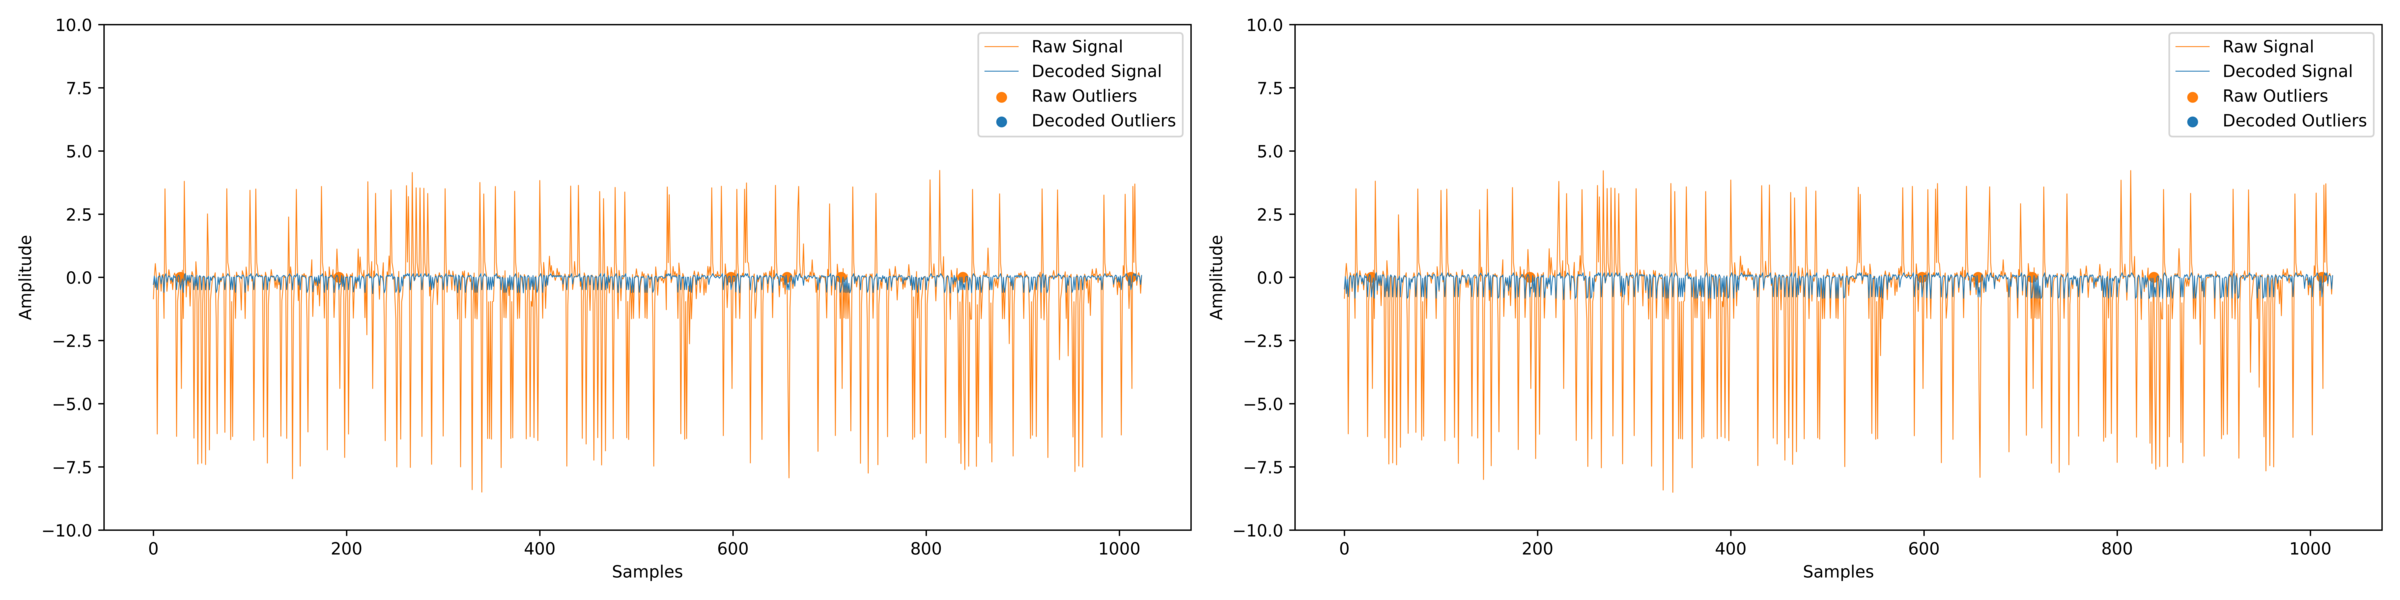
\includegraphics[width=0.8\textwidth]{static/original_vs_decoded_blend_01_resized.png}
%     \caption{Signals when blend=0.1}
%     \label{fig:signal_01}
% \end{figure}
% %
% When the blend is set to 0.8, the decoded signal captures the patterns and flow of the original signal more accurately, with amplitudes reaching up to approximately $\pm0.5$. This improvement demonstrates that increasing the focus on the mean in the loss function results in an overall better reconstruction of the original signal.
% %
% \begin{figure}[ht]
%     \centering
%     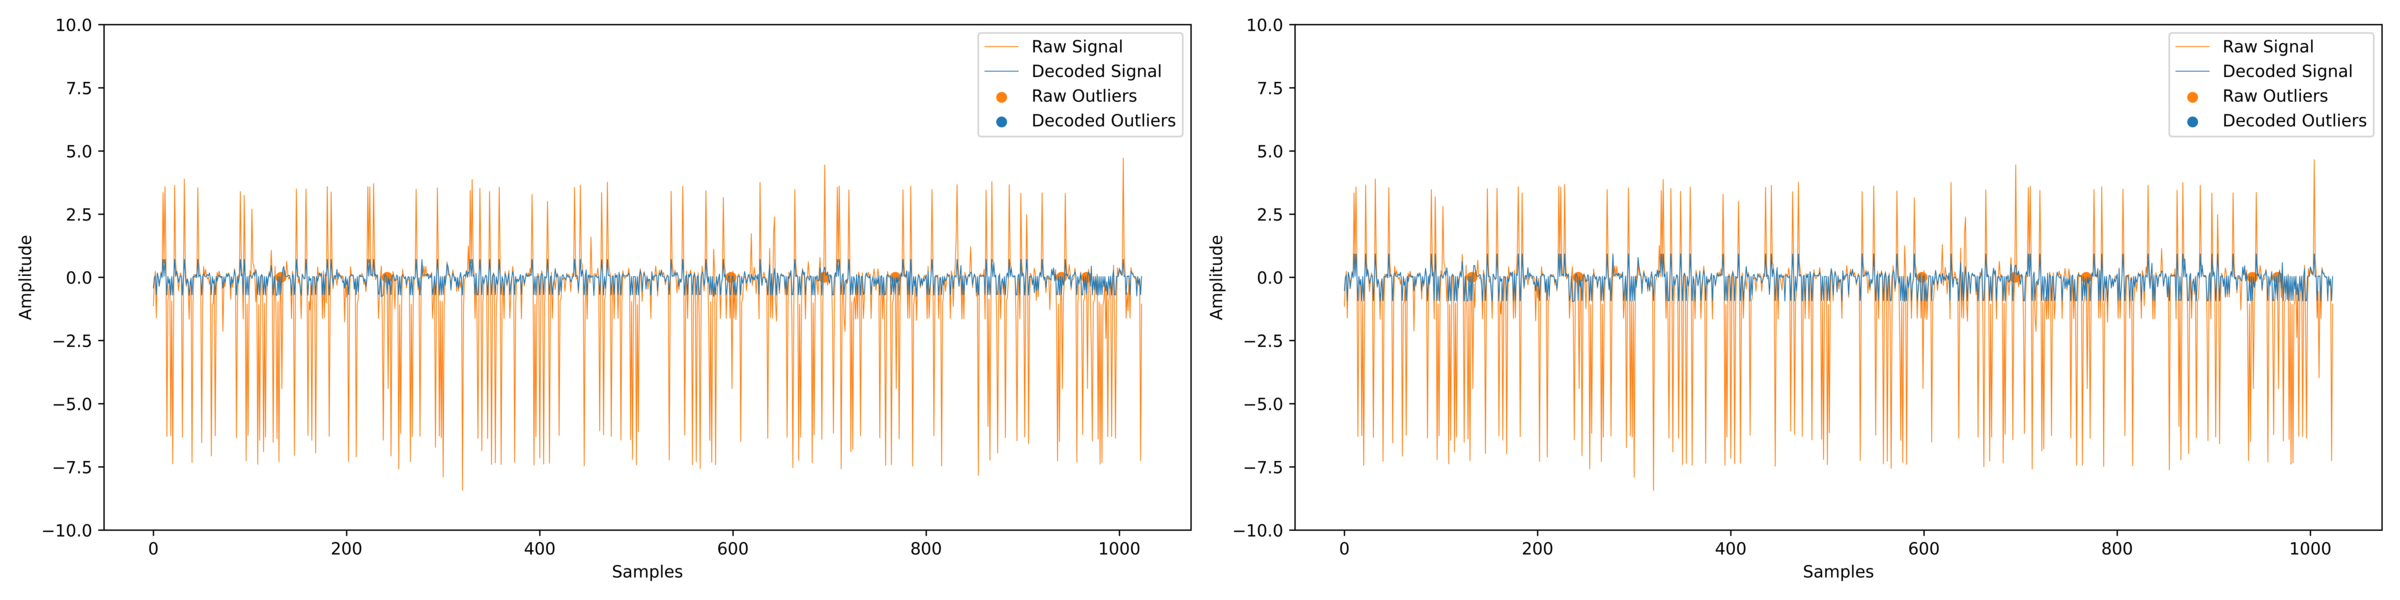
\includegraphics[width=0.8\textwidth]{static/original_vs_decoded_blend_08_resized.png}
%     \caption{Signals when blend=0.8}
%     \label{fig:signal_08}
% \end{figure}
% %

% \subsubsection{Detrended Signal Comparison} We also analyze the detrended signal using the Theil-Sen estimator. For both the 0.1 and 0.8 blends, the detrended signal trends are nearly flat, indicating minimal differences between the original and decoded signals.
% %
% \begin{figure}[ht]
%     \centering
%     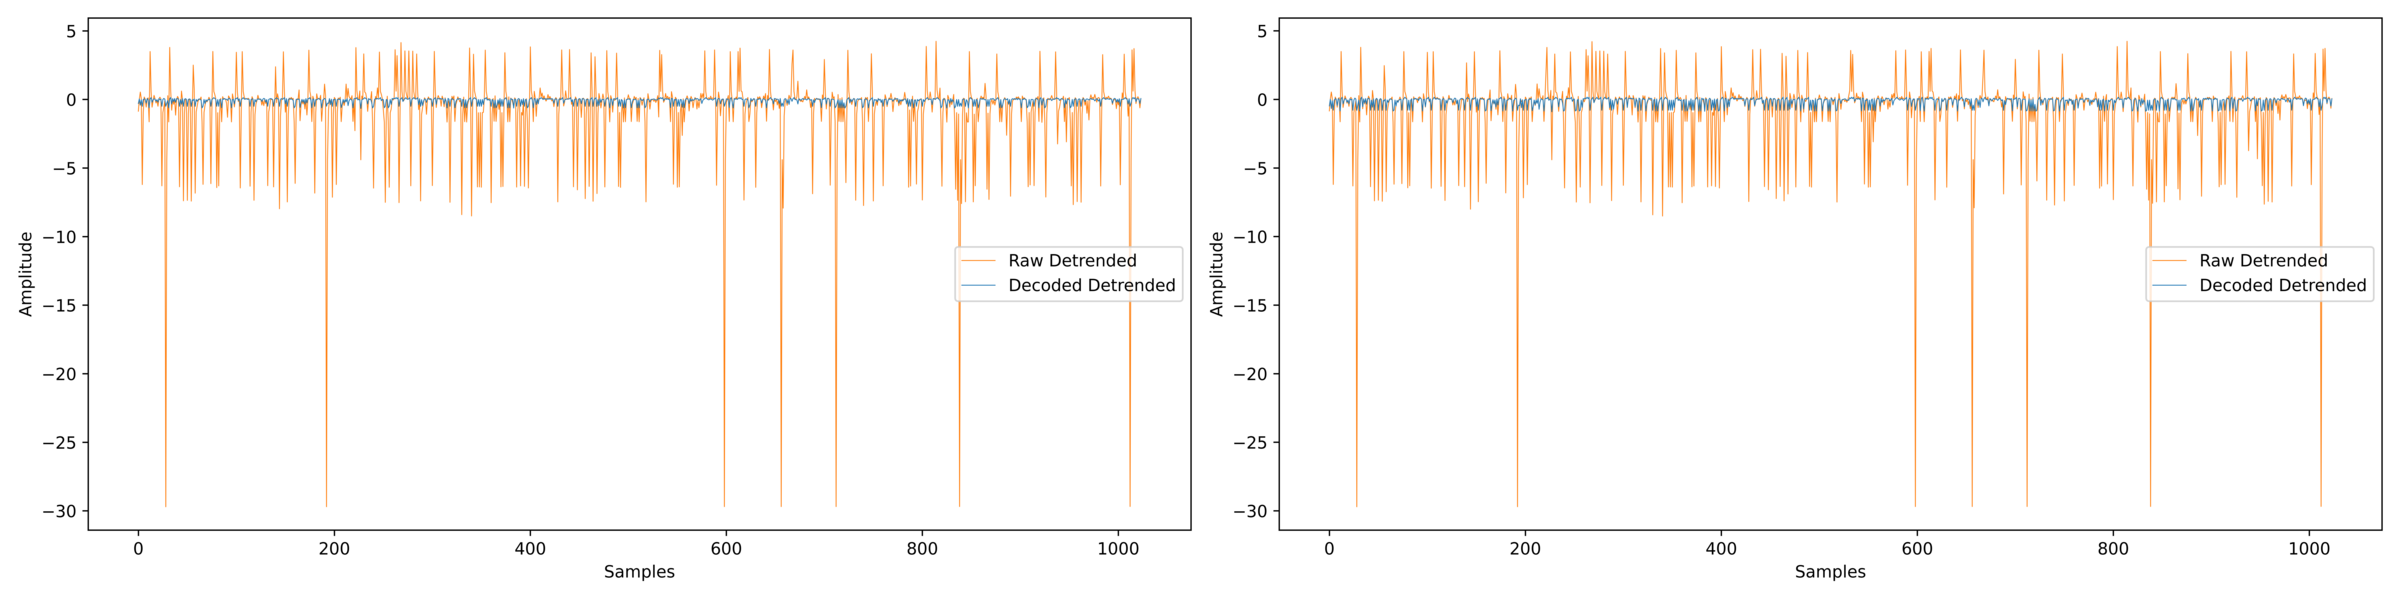
\includegraphics[width=0.8\textwidth]{static/detrended_signal_blend_01_resized.png}
%     \caption{Detrended signals when blend=0.1}
%     \label{fig:detrended_signal_01}
% \end{figure}
% %

% %
% \begin{figure}[ht]
%     \centering
%     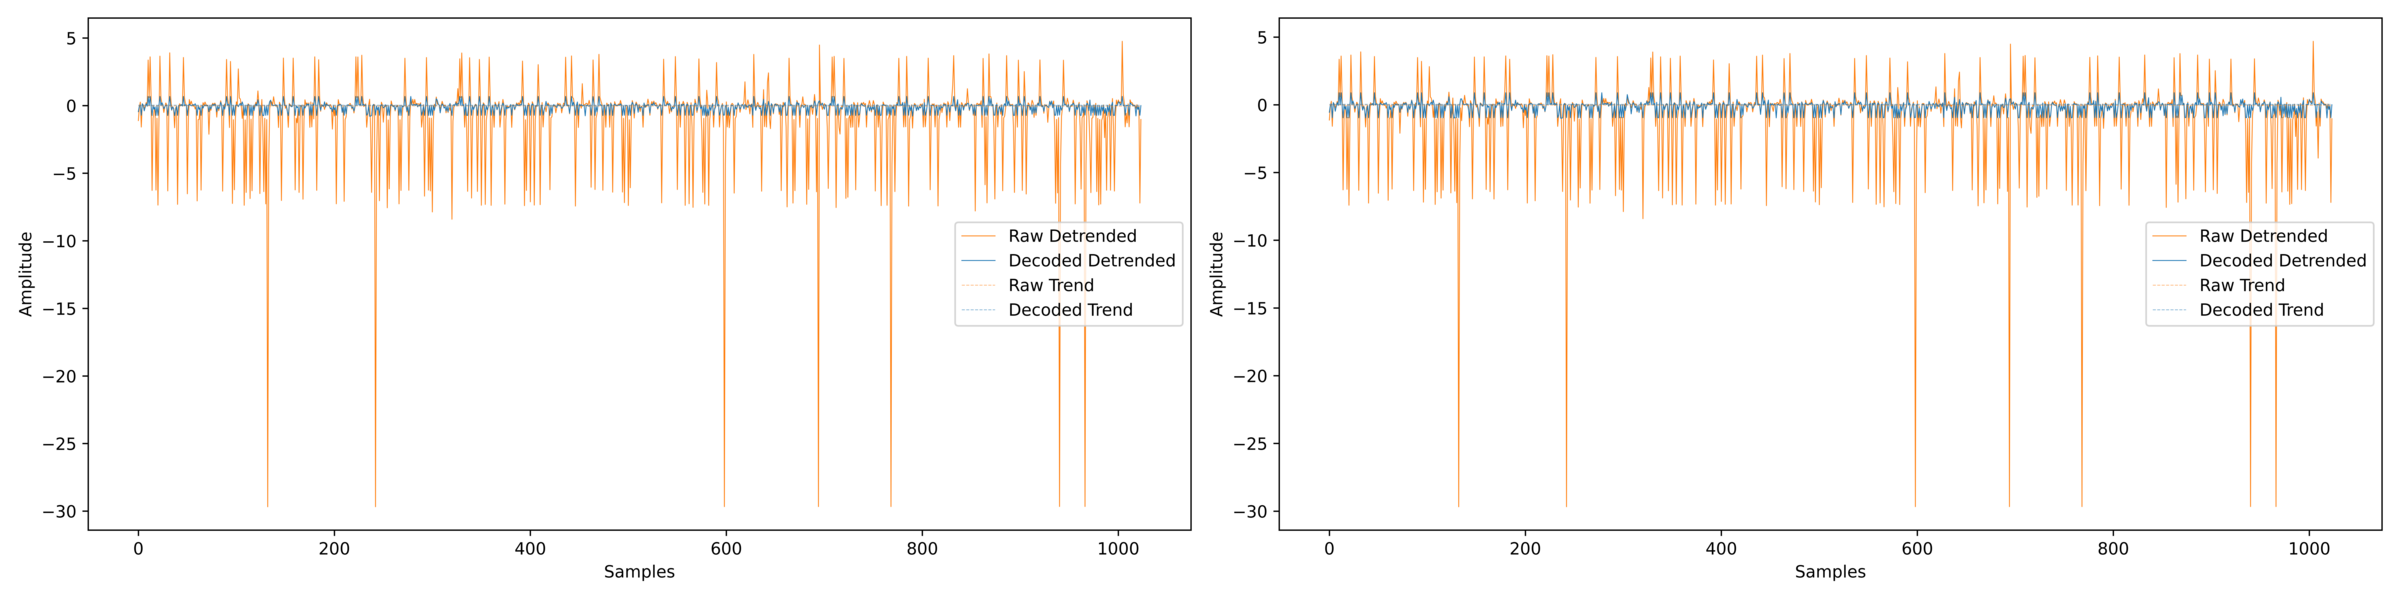
\includegraphics[width=0.8\textwidth]{static/detrended_signal_blend_08_resized.png}
%     \caption{Detrended signals when blend=0.8}
%     \label{fig:detrended_signal_08}
% \end{figure}
% %

% \subsubsection{RMS Analysis} The root mean square (RMS) analysis provides additional insight into the performance of the autoencoder. When the blend is set to 0.1, the majority of the RMS values are centered around zero, with outliers remaining prominent. This result is acceptable but suggests room for improvement. When the blend is set to 0.8, the RMS shows significant improvement, with a higher count of zeros. The outliers continue to exhibit significant values, but overall, the analysis indicates a better reconstruction.
% %
% \begin{figure}[ht]
%     \centering
%     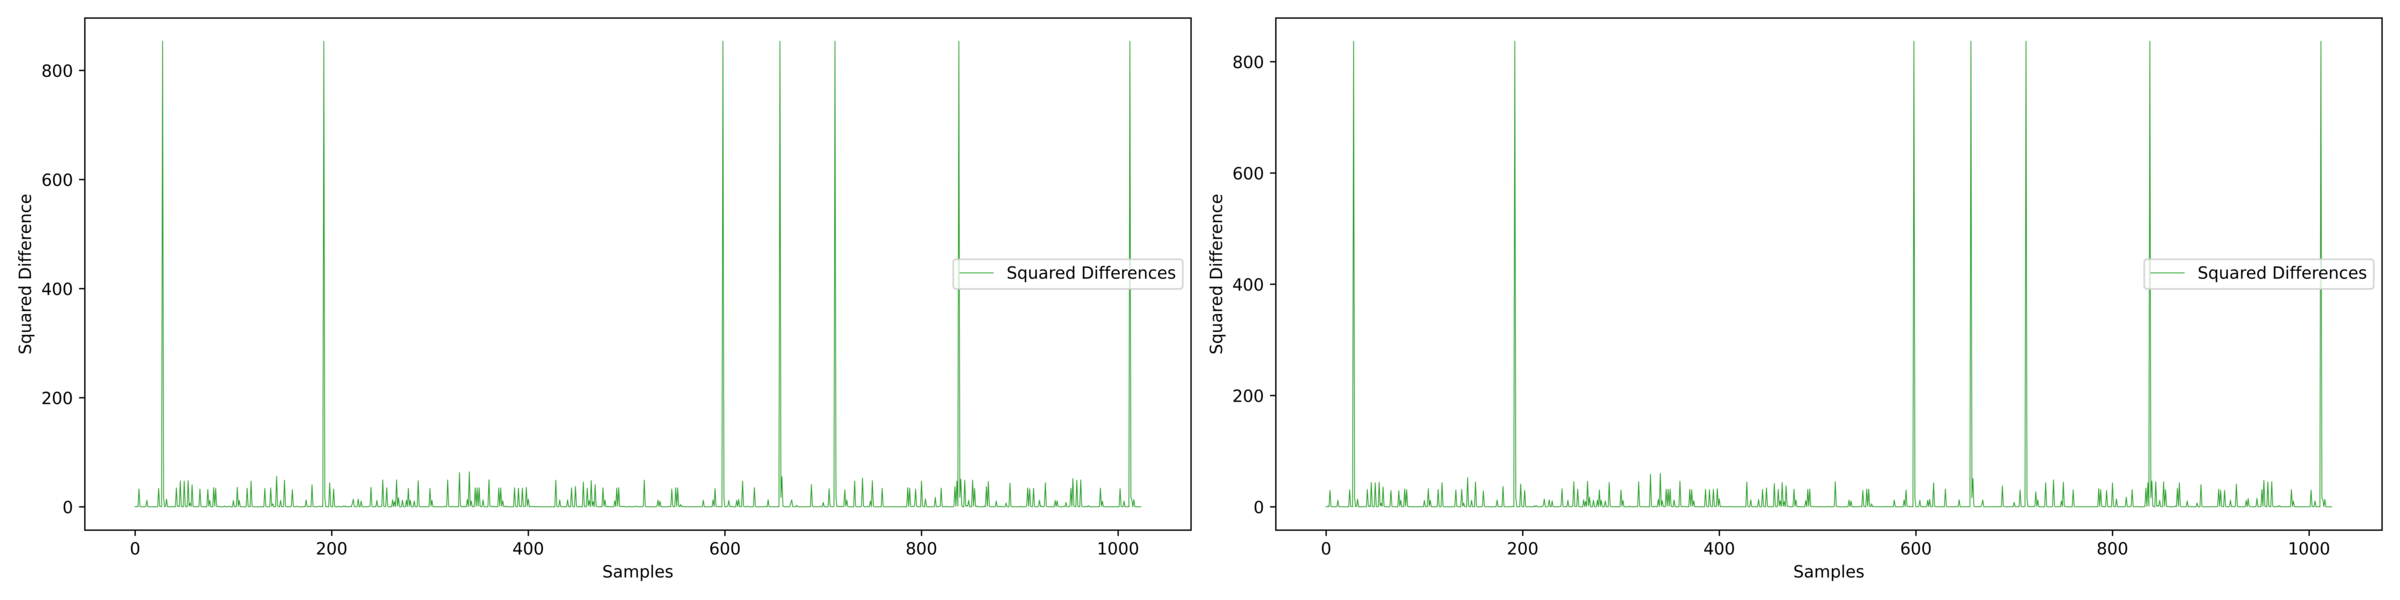
\includegraphics[width=0.8\textwidth]{static/rms_analysis_blend_01_resized.png}
%     \caption{RMS analysis when blend=0.1}
%     \label{fig:rms_analysis_01}
% \end{figure}
% %

% %
% \begin{figure}[ht]
%     \centering
%     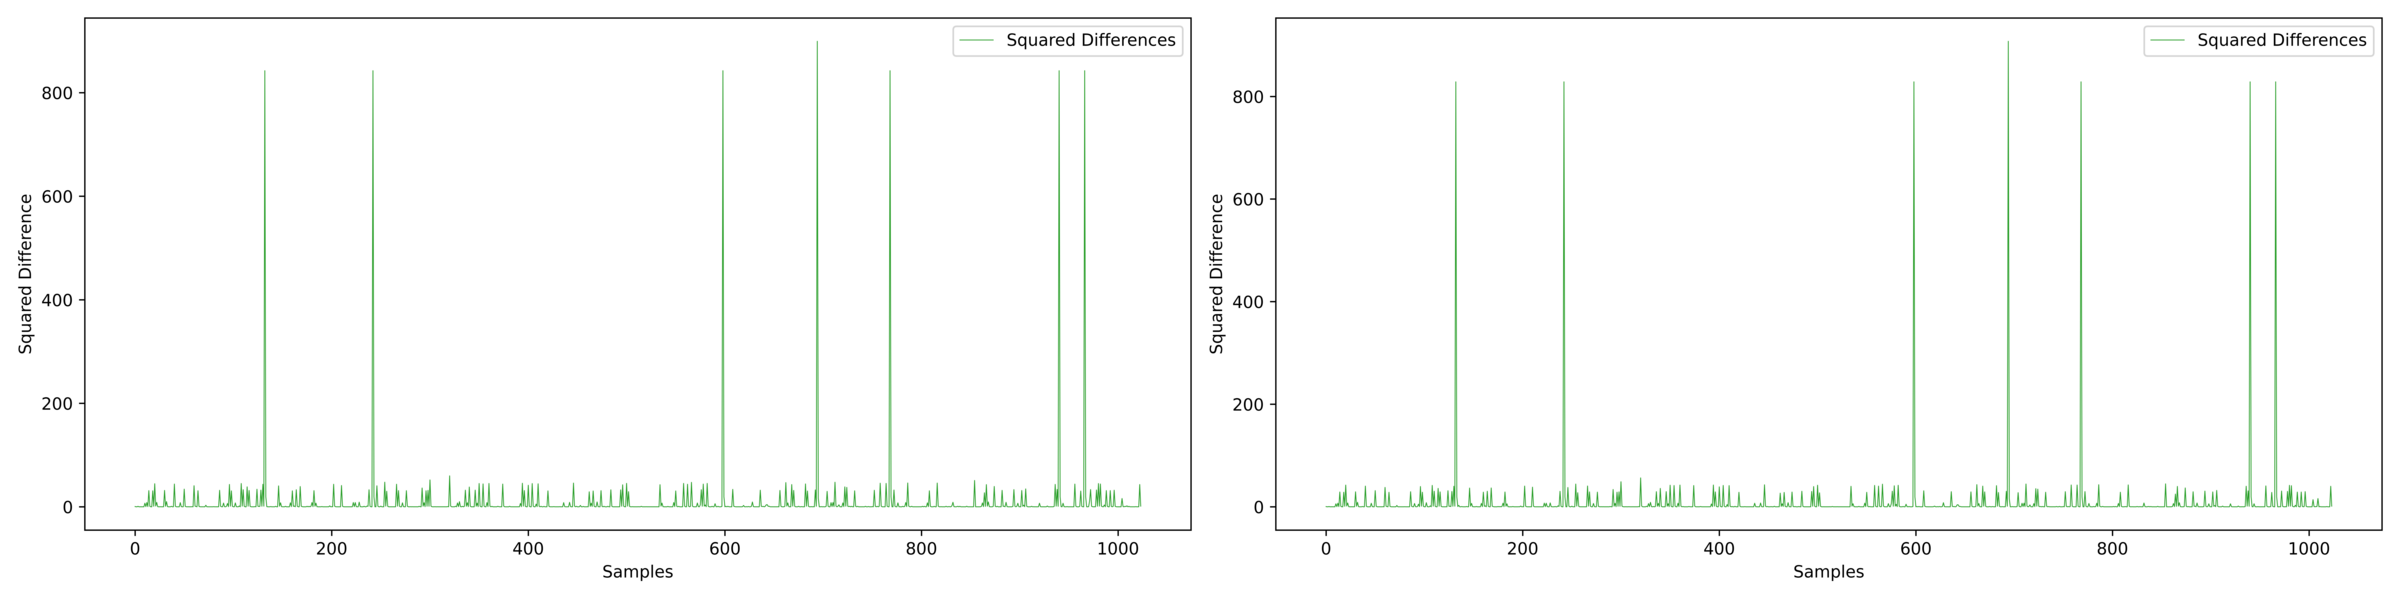
\includegraphics[width=0.8\textwidth]{static/rms_analysis_blend_08_resized.png}
%     \caption{RMS analysis when blend=0.8}
%     \label{fig:rms_analysis_08}
% \end{figure}
% %

% \subsubsection{Band Analysis} When the blend is set to 0.8, the decoded signal exhibits non-zero values across all bands, indicating a more robust amplitude representation. In some bands, the levels of the decoded signal closely match those of the original signal, suggesting that the model effectively captures the corresponding frequency ranges. In contrast, when the blend is set to 0.1, the distributions of the raw and decoded bands differ significantly. Some bands in the decoded signal are nearly zero, while the raw signal contains substantial values, indicating that the amplitude is not well captured.
% %
% \begin{figure}[ht]
%     \centering
%     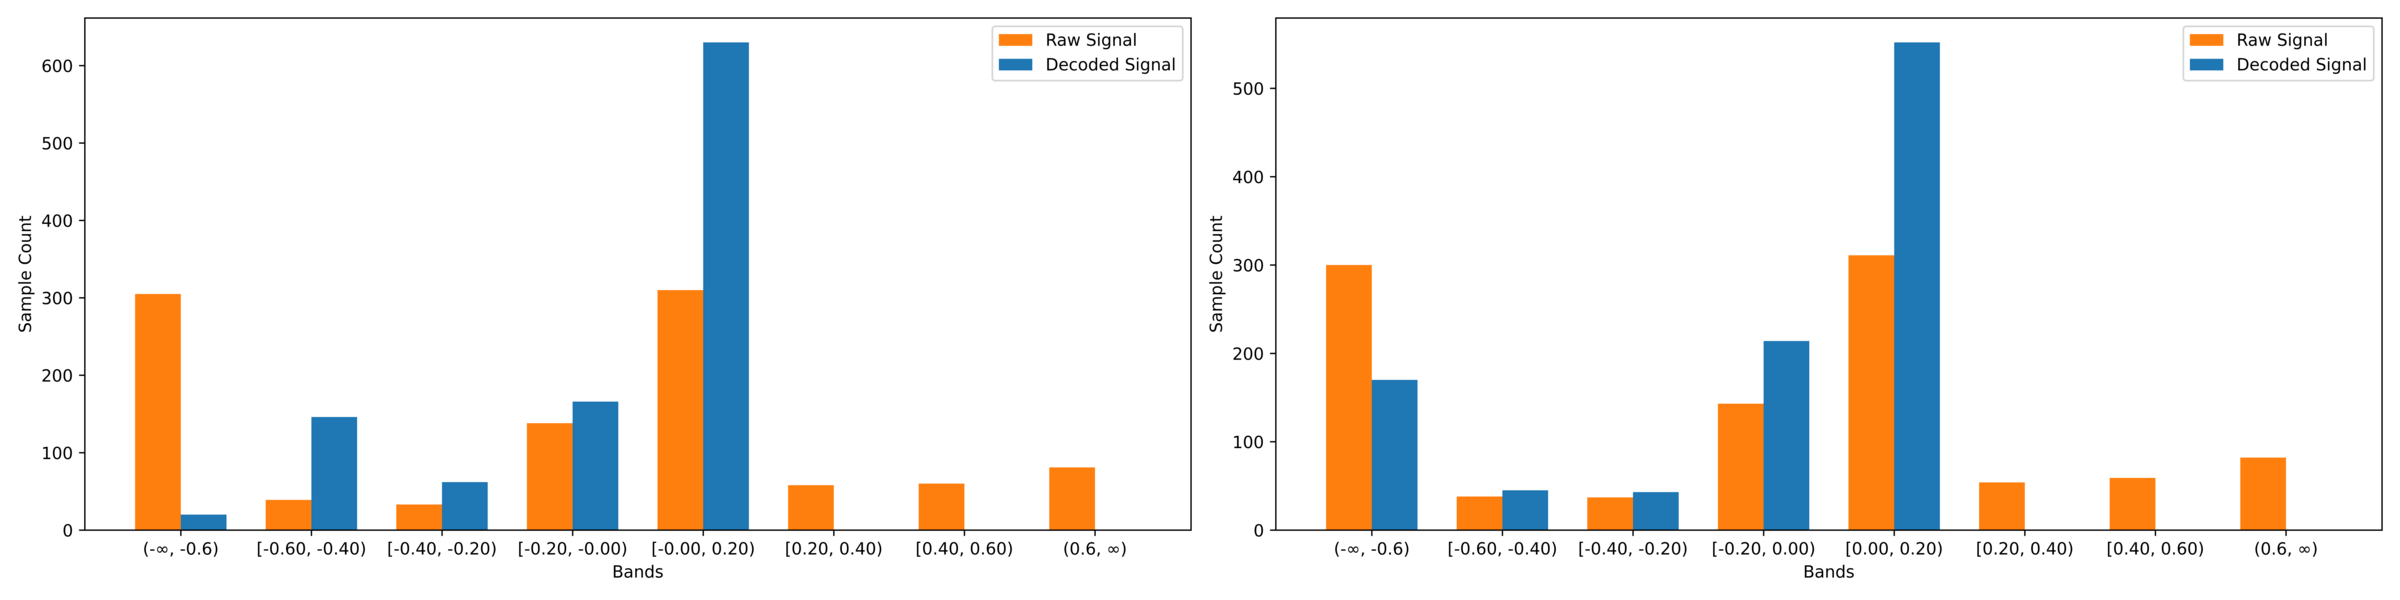
\includegraphics[width=0.8\textwidth]{static/band_analysis_blend_01_resized.png}
%     \caption{Band analysis when blend=0.1}
%     \label{fig:band_analysis_01}
% \end{figure}
% %

% %
% \begin{figure}[ht]
%     \centering
%     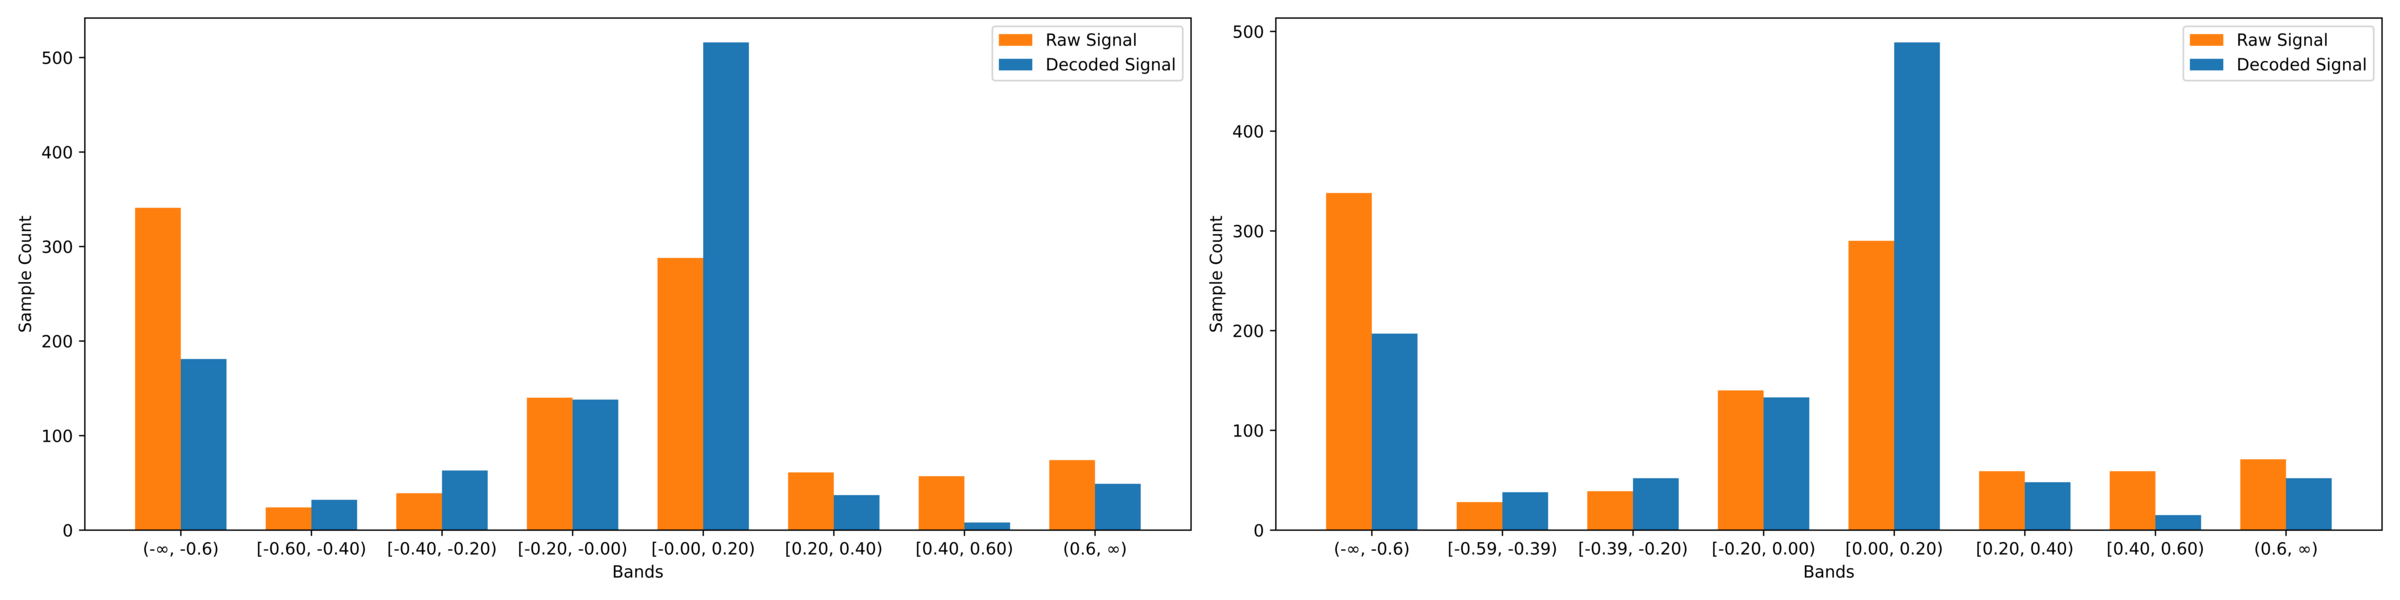
\includegraphics[width=0.8\textwidth]{static/band_analysis_blend_08_resized.png}
%     \caption{Band analysis when blend=0.8}
%     \label{fig:band_analysis_08}
% \end{figure}
% %

% \subsubsection{Other Metrics}

% The performance of the autoencoder is evaluated using various metrics for both blends (0.1 and 0.8). These metrics include band rate differences, zero-crossing rates, RMS values, and Pearson correlation coefficients, calculated as differences between the raw and decoded signals. A smaller difference indicates a closer match to the original signal, which is preferable. Better results are highlighted in blue. Below are the detailed results for each feature and blend setting, showing that the blend with 0.8 is superior.
% %
% \begin{table}[ht]
%     \centering
%     \begin{tabular}{l|c|c}
%         \hline
%         \textbf{Metric} & \textbf{Blend=0.8} & \textbf{Blend=0.1} \\ 
%         \hline
%         Bands \% $F_1$ & 
%         \begin{tabular}[c]{@{}c@{}} 
%         \color{blue}{0.4422} \\ 
%         1.0 \\ 
%         1.0 \\ 
%         -0.1232 \\ 
%         \color{blue}{0.3420} \\ 
%         1.0 \\ 
%         1.0 \\ 
%         \color{blue}{0.3108} 
%         \end{tabular} 
%         & 
%         \begin{tabular}[c]{@{}c@{}} 
%         0.9557 \\ 
%         1.0 \\ 
%         1.0 \\ 
%         \color{blue}{-0.2767} \\ 
%         0.7927 \\ 
%         1.0 \\ 
%         1.0 \\ 
%         1.0 
%         \end{tabular} \\
%         \hline
        
%         Bands \% $F_2$ & 
%         \begin{tabular}[c]{@{}c@{}} 
%         \color{blue}{0.3659} \\ 
%         1.0 \\ 
%         1.0 \\ 
%         \color{blue}{-0.0824} \\ 
%         \color{blue}{0.2217} \\ 
%         1.0 \\ 
%         1.0 \\ 
%         \color{blue}{0.2556} 
%         \end{tabular} 
%         & 
%         \begin{tabular}[c]{@{}c@{}} 
%         0.4524 \\ 
%         1.0 \\ 
%         1.0 \\ 
%         -0.2741 \\ 
%         0.7840 \\ 
%         1.0 \\ 
%         1.0 \\ 
%         1.0 
%         \end{tabular} \\
%         \hline

%         Zero Crossing Rate $F_1$ & 1.3439 & \color{blue}{1.2631} \\ 
 
%         Zero Crossing Rate $F_2$ & 1.3334 & \color{blue}{1.0186} \\ 
 
%         RMS $F_1$ & \color{blue}{2.8682} & 2.9533 \\ 

%         RMS $F_2$ & \color{blue}{2.7980} & 2.8774 \\ 
  
%         Pearson Correlation $F_1$ & \color{blue}{0.6527} & 0.6085 \\ 
   
%         Pearson Correlation $F_2$ & \color{blue}{0.6610} & 0.6364 \\ 
%         \hline
%     \end{tabular}
%     \caption{Comparison of Metrics for Blends 0.1 and 0.8. Metrics are expressed as differences between Raw and Decoded signals.}
%     \label{tab:metrics_comparison}
% \end{table}
% %